\documentclass[journal]{IEEEtran}
\usepackage[a5paper, margin=10mm, onecolumn]{geometry}
\usepackage{tfrupee}
\usepackage{amsmath, amssymb, amsfonts, amsthm}
\usepackage{algorithmic}
\usepackage{graphicx}
\usepackage{textcomp}
\usepackage{xcolor}
\usepackage{txfonts}
\usepackage{listings}
\usepackage{enumitem}
\usepackage{mathtools}
\usepackage{gensymb}
\usepackage{comment}
\usepackage[breaklinks=true]{hyperref}
\usepackage{tkz-euclide} 
\usepackage{listings}
\usepackage[latin1]{inputenc}                                
\usepackage{color}                                            
\usepackage{array}                                            
\usepackage{longtable}                                       
\usepackage{calc}                                             
\usepackage{multirow}                                         
\usepackage{hhline}                                           
\usepackage{ifthen}                                           
\usepackage{lscape}
\newcommand{\myvec}[1]{\begin{pmatrix} #1 \end{pmatrix}}

\begin{document}

\bibliographystyle{IEEEtran}
\vspace{3cm}

\title{NCERT-10.4.2.4}
\author{EE24BTECH11042 - SRUJANA}
{\let\newpage\relax\maketitle}

\renewcommand{\thefigure}{\theenumi}
\renewcommand{\thetable}{\theenumi}
\setlength{\intextsep}{10pt} 

\numberwithin{equation}{enumi}
\numberwithin{figure}{enumi}
\renewcommand{\thetable}{\theenumi}

\textbf{QUESTION}:

Find the two consecutive positive integers, the sum of whose square is 365

\textbf{Theoretical Solution}:\\

\textbf{Simplify the Equation:}
\begin{align}
  x^2 + (x+1)^2 &= 365\\
  2x^2 + 2x + 1 &= 365\\
  2x^2 + 2x &= 364\\
  x^2 + x &= 182
\end{align}

\textbf{Fixed Point Iteration:}

Rearrange the equation as x=g(x) to create an iterative formula:
\begin{align}
    x &= 182 - x^2\\
    x_{n+1} &= g(x_n)\\
    x_{n+1} &= 182 - x_n^2
\end{align}

Select an initial guess x0

However, it is observed that for any initial value x0, the iterative process diverges, 

with the values tending toward -$\infty$. Therefore, this method is unsuitable.\\

\textbf{Newton's Method}

Newton's formula :
\begin{align}
    x_{n+1} &= x_n - \frac{f(x_n)}{f'(x_n)}\\
    f(x) &= x^2 + x - 182\\
    f'(x) &= 2x + 1\\
    x_{n+1} &= x_n - \frac{x_n^2 + x_n - 182}{2x_n + 1}
\end{align}

Choose an initial guess, x0. Since the equation involves a square term, we estimate x0 around $\sqrt{182} \approx 13.5 $

Compute \(x_1, x_2, \dots,\) until \(\lvert x_{n+1} - x_n \rvert < \epsilon\), where \(\epsilon\) is the tolerance (e.g., \(10^{-6}\)).\\

\textbf{Secant Method:}

Unlike Newton's method, the derivative is approximated using two initial points:
\begin{align}
   x_{n+1} &= x_n - f(x_n) \cdot \frac{x_n - x_{n-1}}{f(x_n)-f(x_{n+1})}\\
\end{align}

Start with two initial guesses, such as x0=13.5 and x1=14, and iterate until convergence.

\textbf{Eigen values of companion matrix}

In this method, we find the roots of any polynomial of the form \(x^n + a_{n-1}x^{n-1}\dots ax+a_0=0\) by finding the eigenvalues of the Companion Matrix \(C\) given below:
\begin{align}
    C &= \myvec{0&1&0&\dots&0\\ 0&0&1&\dots&0\\ \vdots &\vdots &\vdots &\ddots&\vdots\\0&0&0&\vdots&1\\-a_0&-a_1&-a_2&\dots&-a_{n-1}}
\end{align}
For the Quadratic Equation \(x^2 + x = 182\), we get the following companion Matrix
\begin{align}
    C&=\myvec{0&1\\182&-1}
\end{align}
The roots of the equation are the eigenvalues of the matrix \(C\), which have been calculated using the QR Decomposition with shifts process:

\textbf{QR algorithm:}

In the QR algorithm, the matrix \(A_n\) is decomposed into matrices \(Q_n\) and \(R_n\) as:
\begin{align}
    A_{n}&=Q_nR_n
\end{align}
Then, the new matrix \(A_{n+1}\) is computed as:
\begin{align}
    A_{n+1}&=R_nQ_n
\end{align}
This process is repeated until the off-diagonal elements of the matrix become negligibly small, at which point the diagonal elements approximate the eigenvalues of the original matrix.

Eigenvalues computed: [13.0 , -14.0]

we should consider only positive integer i.e .. 13


\begin{figure}[h!]
   \centering
   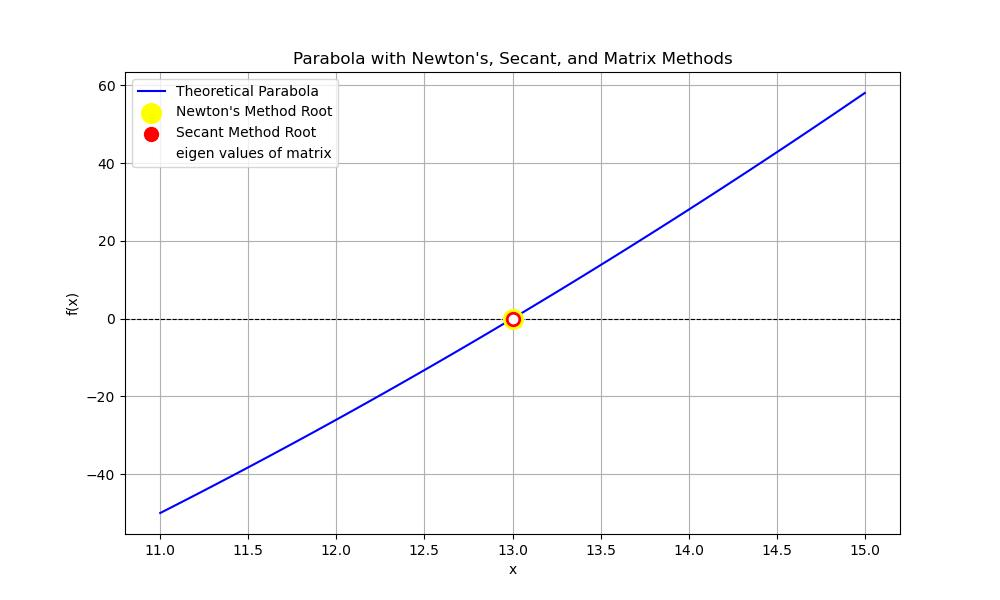
\includegraphics[width=\columnwidth]{fig/combined_fig.jpg}
\end{figure}
\end{document}

